\chapter{Direct reinforcement learning of decision tree policies}\label{sec:topin}
In this chapter, we compare deep reinforcement learning--direct learning--of decision tree policies (cf. chapter~\ref{sec:intro-pomdp}) to imitation learning--indirect learning--of decision tree policies (cf. section~\ref{sec:imit}).
In particular, we attempt to reproduce the results from~\cite[table 1]{topin2021iterative} in which authors compare direct and indirect learning of decision tree policies of depth at most 2 for the CartPole MDP~\cite{cartpole}.
In the original paper, authors find that both direct and indirect learning yields decision tree policies with similar RL objective values (cf. definition~\ref{def:mdp-obj}) for the CartPole.
On the other hand, we find that, imitation learning, despite not directly optimizing the RL objective for CartPole, outperforms deep RL that optimizes the interpretable RL objective (cf. definition~\ref{def:irl} in which the objective trades off the standard RL objective and interpretability).

\section{Reproducing ``Iterative Bounding MDPs: Learning Interpretable Policies via Non-Interpretable Methods''}

Authors of \cite{topin2021iterative} use two deep reinforcement learning baselines (cf. section~\ref{sec:drl}) to which they apply some modifications in order to learn partially observable policies as required by proposition \ref{def:po-policy} and by the interpretable RL objective (cf. definition~\ref{def:irl}).
Authors modify the standard DQN (cf. algorithm~\ref{alg:dqn}) to return a partially observable policy. The trained $Q$-function is approximated with a neural network $O\rightarrow \mathbb{R}^{|A\cup A_{info}|}$ rather than $S\times O\rightarrow \mathbb{R}^{|A\cup A_{info}|}$.
In this modified DQN, the temporal difference error target for the $Q$-function $O\rightarrow A\cup A_{info}$ is approximated by a neural network $S\times O\rightarrow A\cup A_{info}$ that is in turn trained by bootstrapping the temporal difference error with itself.
We present the modifications in algorithm~\ref{alg:mod-dqn}.
Similar modifications are applied to the standard PPO (cf. algorithm~\ref{alg:ppo}) that we present in the appendix (cf. algorithm \ref{alg:mod-ppo}). In the modified PPO, neural network policy $O\rightarrow A\cup A_{info}$ is trained using a neural network value function $S\times O\rightarrow A\cup A_{info}$ as a critic.

Those two variants of DQN and PPO have first been introduced in \cite{pinto} for robotic tasks with partially observable components, under the name ``asymmetric'' actor-critic. 
Asymmetric RL algorithms that have policy and value estimates using different information from a POMDP~\cite{POMDP,chap2} were later studied theoretically to solve POMDPs in Baisero's work~\cite{baisero-dqn,baisero-ppo}.
The connections from Deep RL in IBMDPs for objective is absent from \cite{topin2021iterative} and we defer their connections to direct interpretable reinforcement learning to the next chapter as our primary goal is to reproduce \cite{topin2021iterative} \textit{as is}.
Next, we present the precise experimental setup we use to reproduce~\cite[table 1]{topin2021iterative} in order to study direct deep reinforcement learning of decision tree policies for the CartPole MDP.

\begin{algorithm}
    \KwData{IBMDP $\mathcal{M}_{IB}\langle S\times O, A\cup A_{info}, (R, \zeta),( T, T_0, T_{info})\rangle$, learning rate $\alpha$, exploration rate $\epsilon$, partially observable Q-network parameters $\theta$, Q-network parameters $\phi$, replay buffer $\mathcal{B}$, update frequency $C$}
    \KwResult{Partially observable deterministic policy $\pi_{po}$}
    Initialize partially observable Q-network parameters $\theta$\\
    \textcolor{green}{Initialize Q-network parameters $\phi$ and target network parameters $\phi^- = \phi$} \\

    Initialize replay buffer $\mathcal{B} = \emptyset$ \\
    \For{each episode}{
        Initialize base state features $\boldsymbol{s}_0 \sim T_0$ \\
        Initialize observation $\boldsymbol{o}_0 = (L_1, U_1, \dots, L_p, U_p)$ \\

        \For{each step $t$}{
            Choose action $a_t$ using $\epsilon$-greedy: $a_t = \operatorname{argmax}_a Q_\theta(\boldsymbol{o}_t,a)$ with prob. $1-\epsilon$ \\
            Take action $a_t$, observe $r_t$ \\
            Store transition $(\boldsymbol{s}_t, \boldsymbol{o}_t, a_t, r_t, \boldsymbol{s}_{t+1})$ in $\mathcal{B}$ \\
            Sample random batch $(\boldsymbol{s}_i, \boldsymbol{o}_i, a_i, r_i, \boldsymbol{s}_{i+1}) \sim \mathcal{B}$ \\
            $a' = \underset{a}{\operatorname{argmax}} Q_{\theta}(\boldsymbol{o}_i, a)$ \\
            \textcolor{green}{$y_i = r_i + \gamma Q_{\phi^-}(\boldsymbol{s}_{i+1}, a')$} \Comment{// Compute target}
            $\phi \leftarrow \phi - \alpha \nabla_\phi (Q_\phi(\boldsymbol{s}_i, a_i) - y_i)^2$ \Comment{// Update Q-network}
            \textcolor{green}{$\theta \leftarrow \theta - \alpha \nabla_\theta (Q_\theta(\boldsymbol{o}_i, a_i) - y_i)^2$} \Comment{// Update partially observable Q-network}

            \If{$t \bmod C = 0$}{
                $\theta^- \leftarrow \theta$ \Comment{// Update target network}
            }
            $\boldsymbol{s}_t \leftarrow \boldsymbol{s}_{t+1}$ \\
            $\boldsymbol{o}_t \leftarrow \boldsymbol{o}_{t+1}$ \\
        }
    }
    $\pi_{po}(\boldsymbol{o}) = \operatorname{argmax}_a Q_\theta(\boldsymbol{o},a)$ \Comment{// Extract greedy policy}
    \caption{Modified Deep Q-Network. We highlight in green the changes to the standard DQN (cf. algorithm~\ref{alg:dqn}).}\label{alg:mod-dqn}
\end{algorithm}

\section{Experimental setup}
\subsection{(IB)MDP} 

We use the exact same base MDP and associated IBMDPs for our experiments as~\cite{topin2021iterative} except when mentioned otherwise.

\paragraph{Base MDP} The task at hand is to optimize the RL objective (cf. definition~\ref{def:mdp-obj}) with a decision tree policy for the CartPole MDP~\cite{cartpole}.
At each time step a learning algorithm observes the cart's position and velocity and the pole's angle and angular velocity, and can take action to push the CartPole left or right.
While the CartPole is roughly balanced, i.e., while the cart's angle remains in some fixed range, the agent gets a positive reward.
If the CartPole is out of balance, the MDP transitions to an absorbing terminal state and gets 0 reward forever.
Like in~\cite{topin2021iterative}, we use the gymnasium \texttt{CartPole-v0} implementation~\cite{gymnasium} of the CartPole MDP in which trajectories are truncated after 200 timesteps making the maximum cumulative reward, i.e. the optimal value of the RL objective when $\gamma=1$, to be 200.
The state features of the CartPole MDP are in $[-2, 2] \times [-2, 2] \times [-0.14, 0.14] \times [-1.4, 1.4]$.

\paragraph{IBMDP} Authors define the associated IBMDP (cf. definition~\ref{def:ibmdp}) with $\zeta=-0.01$ and 4 information gathering actions.
In appendix~\ref{sec:ibmdp-paper}, we give more details about how the authors of the original IBMDP paper chose the information gathering actions.
In addition to the original paper IBMDP, we also try $\zeta=0.01$ and 3 information gathering actions.
We use the same discount factor as the authors: $\gamma=1$.
We try two different approaches to limit the depth of decision tree policies to be at most 2: terminating trajectories if the agent takes too much information gathering in a row or simply giving a reward of $-1$ to the agent every time it takes an information gathering action past the depth limit.
In practice, we could have tried an action masking approach, i.e. having a state dependent actions set, but we want to abide to the MDP formalism in order to properly understand direct interpretable approaches.
We will also try IBMDPs where we do not limit the maximum depth for completeness.


\subsection{Baselines}
\paragraph{Modified DQN and Modified PPO} as mentioned above, authors use the modified version of DQN from algorithm~\ref{alg:mod-dqn}.
We use the exact same hyperparameters for modified DQN as the authors when possible. 
We use the same layers width (128) and number of hidden layers (2), the same exploration strategy ($\epsilon$-greedy with linearly decreasing value $\epsilon$ between 0.5 and 0.05 during the first 10\% of the training),
the same replay buffer size ($10^6$) and the same number of transitions to be collected randomly before doing value updates ($10^5$).
We also try to use more exploration during training (change the initial $\epsilon$ value to 0.9).
We use the same optimizer (RMSprop with hyperparameter 0.95 and learning rate $2.5 \times 10^{-4}$) to update the $Q$-networks.
Authors did not share which DQN implementation they used so we use the stable-baselines3 one~\cite{stable-baselines3}.
Authors did not share which activation functions they used so we try both $\operatorname{tanh}$ and $\operatorname{relu}$. 
For the modified PPO algorithm (cf. algorithm~\ref{alg:mod-ppo}), we can exactly match the authors hyperparameters since they use the open source stable-baselines3 implementation of PPO.
We match training budgets: we train modified DQN on 1 million timesteps and modified PPO on 4 million timesteps.

\paragraph{DQN and PPO} We also benchmark the standard DQN and PPO when learning standard Markovian IBMDP policies $\pi:S\times O\rightarrow A\cup A_{info}$ and when learning standard $\pi:S\rightarrow A$ policies directly in the CartPole MDP.
We summarize hyperparameters for the IBMDP and for the learning algorithms in appendices~\ref{tab:ibmdp-params}, \ref{tab:ibmdp-rl1} and \ref{tab:ibmdp-rl2}.

\paragraph{Indirect methods} We also compare modified RL algorithm to imitation learning (cf. section \ref{sec:imit}).
To do so, we use VIPER or Dagger (cf. algorithms~\ref{alg:dagger} and~\ref{alg:viper}) to imitate greedy neural network policies obtained with standard DQN learning directly on CartPole.
We use Dagger to imitate neural network policies obtained with the standard PPO learning directly on CartPole. 
For each indirect method, we imitate the neural network experts by fitting decision trees on 10000 expert transitions using the CART (cf. algorithm~\ref{alg:cart}) implementation from scikit-learn~\cite{scikit-learn} with default hyperparameters and maximum depth of 2 like in ~\cite{topin2021iterative}.
    
\subsection{Metrics}
The key metric of this section is performance when controlling the CartPole, i.e, the average \textit{undiscounted} cumulative reward of a policy on 100 trajectories (RL objective with $\gamma=1$).
For modified RL algorithms that learn a partially observable policy (or $Q$-function) in an IBMDP, we periodically extract the policy (or $Q$-function) and use algorithm~\ref{alg:extract-tree} to extract a decision tree for the CartPole MDP. 
We then evaluate the tree on 100 independent trajectories in the MDP and report the mean undiscounted cumulative reward.
For RL applied to IBMDPs, since we can't deploy learned policies directly to the base MDP as the state dimensions mismatch--such policies are $S\times O\rightarrow A \cup A_{info}$ but the MDP states are in $S$--we periodically evaluate those IBMDP policies in a copy of the IBMDP in which we fix $\zeta=0$ ensuring that the copied IBMDP undiscounted cumulative rewards only account rewards from the CartPole MDP (non-zero rewards in the IBMDP only occur when a reward from the base MDP is given, i.e. when $a_t\in A$ in the IBMDP (cf. definition~\ref{def:ibmdp})).
Similarly, we do 100 trajectories of the extracted policies in the copied IBMDP and report the average undiscounted cumulative reward.
For RL applied directly to the base MDP we can just periodically extract the learned policies and evaluate them on 100 CartPole trajectories.

Since imitation learning baselines train offline, i.e, on a fixed dataset, their performances cannot directly be reported on the same axis as RL baselines.
For that reason, during the training of a standard RL baseline, we periodically extract the trained neural policy/$Q$-function that we consider as the expert to imitate.
Those experts are then imitated with VIPER or Dagger using 10 000 newly generated transitions and the fitted decision tree policies are then evaluated on 100 CartPole trajectories.
We do not report the imitation learning objective values during VIPER or Dagger training.
Every single combination of IBMDP and Modified RL hyperparameters is run 20 times.
For standard RL on either an IBMDP or an MDP, we use the paper original hyperparameters when they were specified, with depth control using negative rewards, $\operatorname{tanh()}$ activations.
We use 20 individual random seeds for every experiment in this chapter.
Next, we present our results when reproducing~\cite[table 1]{topin2021iterative}.

\section{Results}

\subsection{How well do modified deep RL baselines learn in IBMDPs?}

\begin{figure}
    \centering
    \begin{subfigure}[b]{0.49\textwidth}
        \centering
        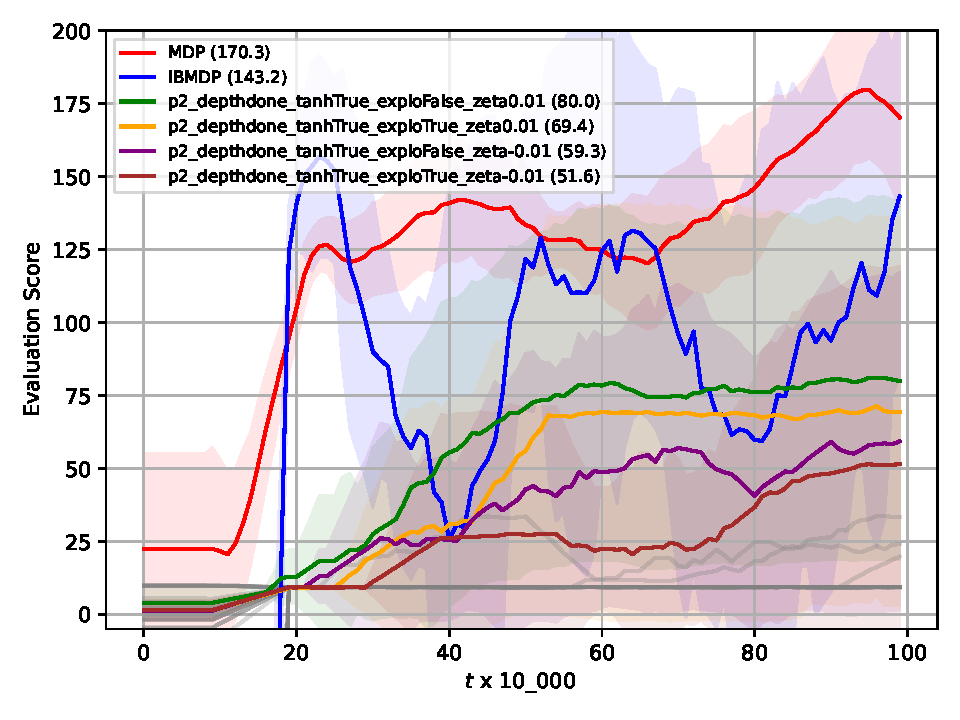
\includegraphics[width=\textwidth]{images/images_part1/dqn.pdf}
        \caption{DQN variants}\label{fig:res-dqn}
    \end{subfigure}
    \hfill
    \begin{subfigure}[b]{0.49\textwidth}
        \centering
        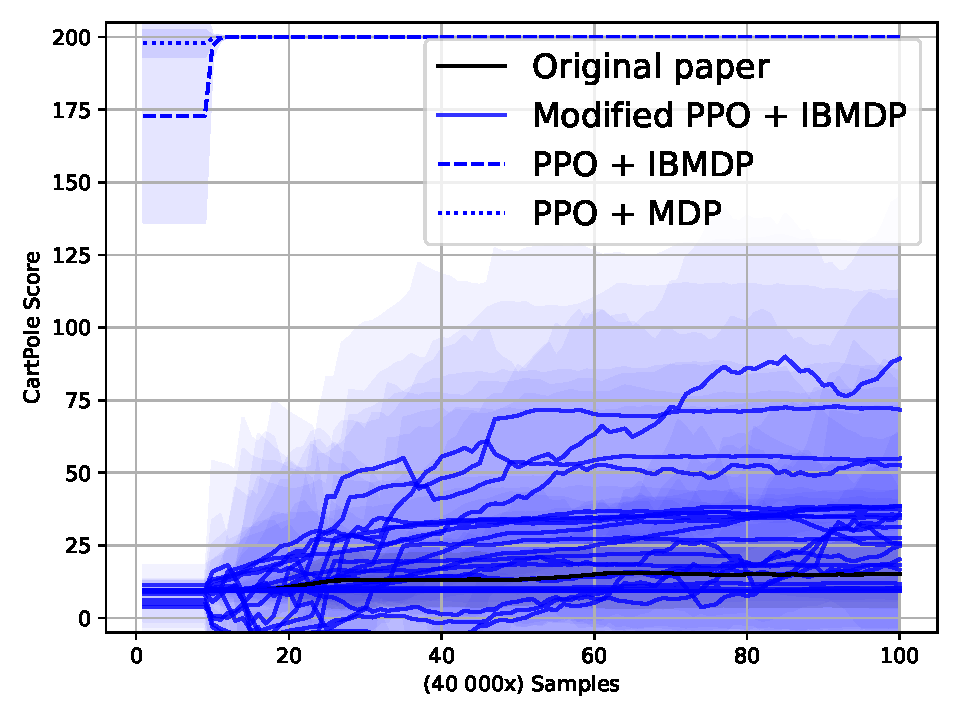
\includegraphics[width=\textwidth]{images/images_part1/ppo.pdf}
        \caption{PPO variants}\label{fig:res-ppo}
    \end{subfigure}
    \caption{Comparison of modified reinforcement learning algorithms on different CartPole IBMDPs. (a) Shows variations of modified DQN and DQN (cf. table~\ref{tab:ibmdp-rl1}), while (b) shows variations of modified PPO and PPO (cf. table~\ref{tab:ibmdp-rl2}). For both algorithms, we give different line-styles for the learning curves when applied directly on the CartPole MDP versus when applied on the IBMDP to learn standard Markovian policies. We color the modified RL algorithm variant from the original paper in black. Shaded areas represent the confidence interval at 95\% at each measure on the y-axis.}
\end{figure}
On figure~\ref{fig:res-dqn}, we observe that modified DQN can learn in IBMDPs--the curves have an increasing trend--but we also observe that modified DQN finds poor decision tree policies for the CartPole MDP in average--the curves flatten at the end of the x-axis and have low y-values.
In particular, the highest final y-value, among all the learning curves that could possibly correspond to the original paper modified DQN, correspond to poor performances on the CartPole MDP.
On figure~\ref{fig:res-ppo}, we observe that modified PPO finds decision tree policies with almost 150 cumulative rewards towards the end of training.
The performance difference with modified DQN could be because we trained modified PPO longer, like in the original paper.
However it could also be because DQN-like algorithms with those hyperparameters struggle to learn in CartPole (IB)MDPs.
Indeed, we notice that for DQN-like baselines, learning seems difficult in general independently of the setting.
On figures~\ref{fig:res-dqn} and~\ref{fig:res-ppo}, we observe that standard RL baselines (RL + IBMDP and RL + MDP), learn better CartPole policies in average than their modified counterparts that learn partially observable policies (cf. proposition~\ref{def:po-policy}). 
On figure~\ref{fig:res-ppo}, it is clear that for the standard PPO baselines, learning is super efficient and algorithms learn optimal policies with reward 200 in few thousands steps.

\subsection{Which decision tree policies does direct reinforcement learning return for the CartPole MDP?}

\begin{figure}
    \centering
    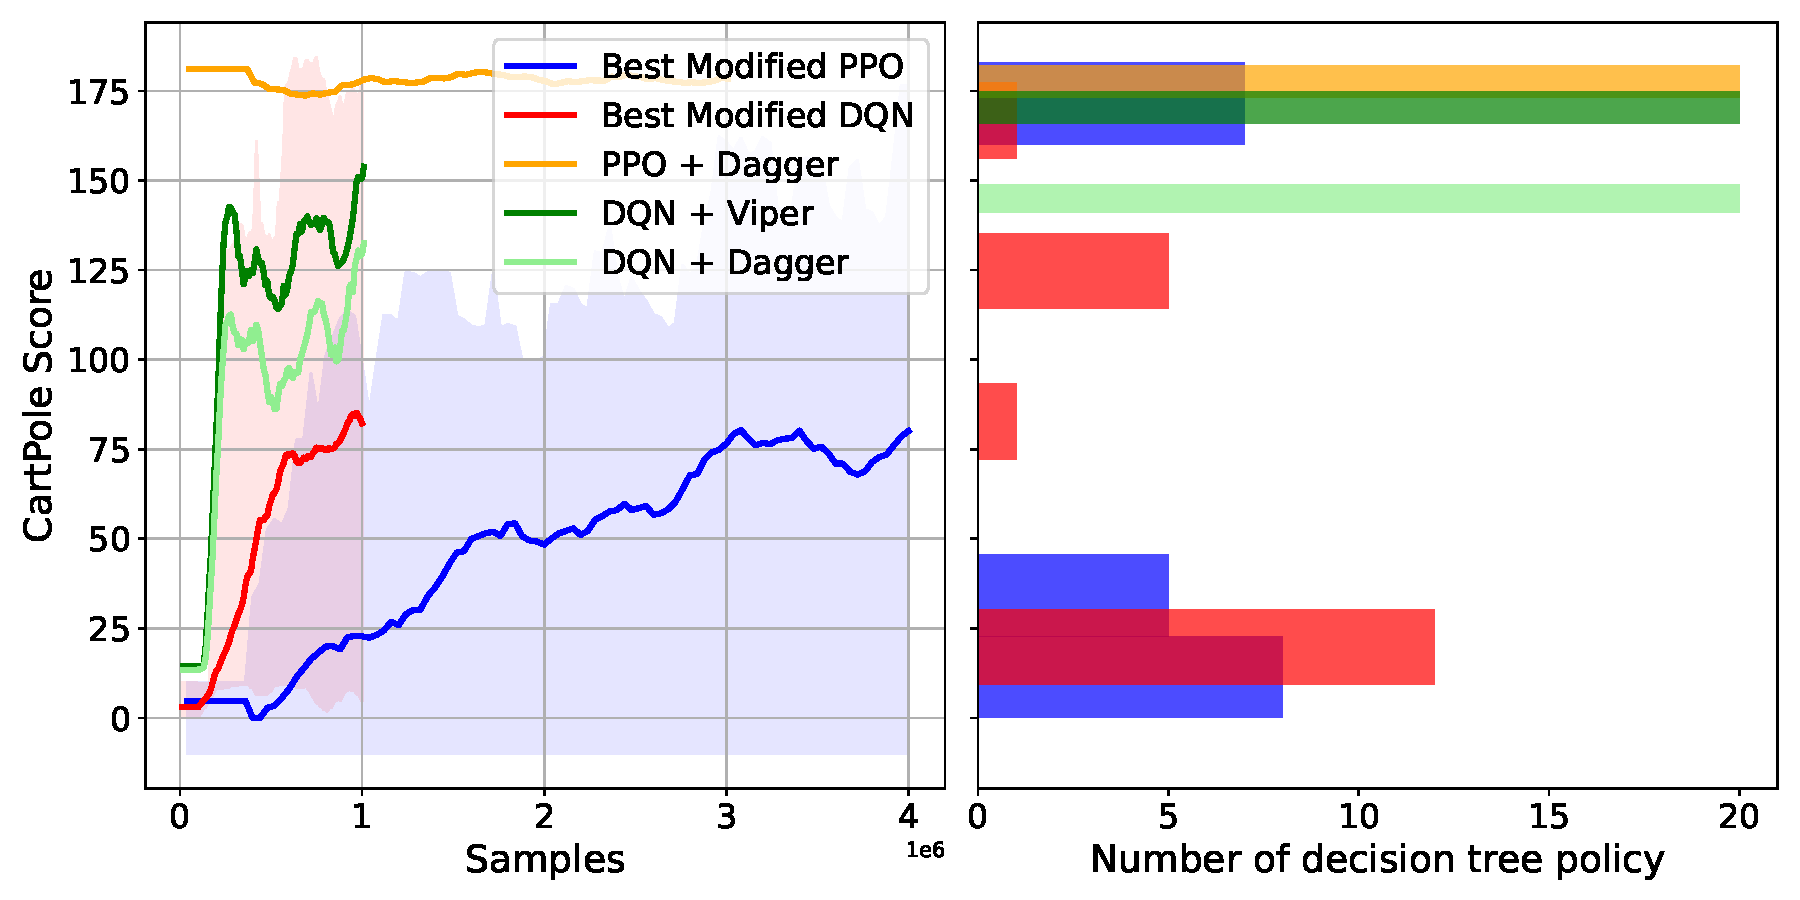
\includegraphics[width=1\textwidth]{images/images_part1/ppo_tree_study.pdf}
    \caption{(left) Mean performance of the best--w.r.t. the RL objective for CartPole--modified RL + IBMDP combination. Shaded areas represent the min and max performance over the 20 seeds during training. (right) Corresponding score distribution of the final decision tree policies w.r.t. the RL objective for CartPole.}\label{fig:ppo-trees}
\end{figure}


\begin{figure}
    \centering
    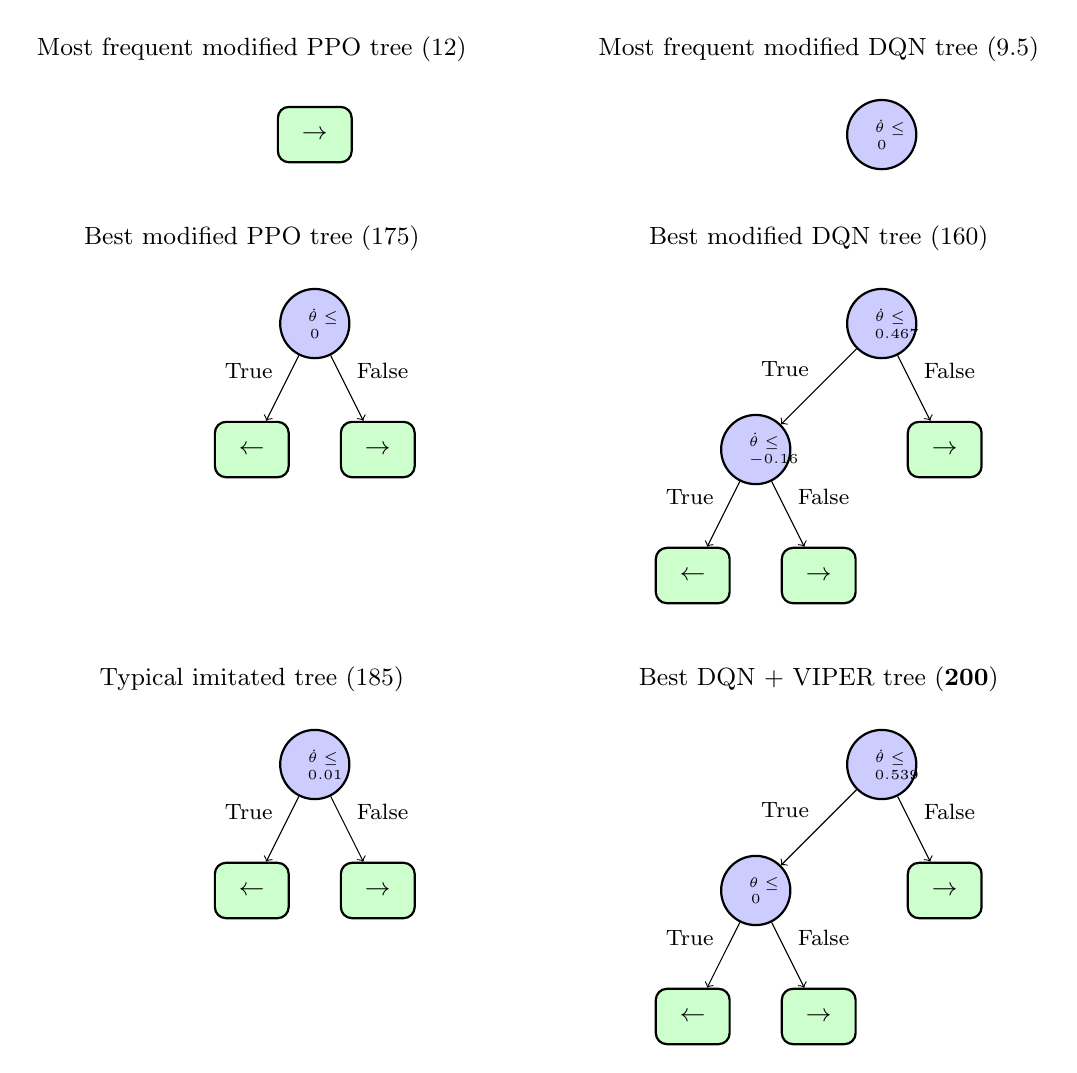
\begin{tikzpicture}[
        scale=0.8,
        decision/.style={circle, draw, thick, fill=blue!20, text width=0.5em, text centered, minimum height=2.5em, font=\tiny},
        leaf/.style={rectangle, draw, thick, fill=green!20, text width=2em, text centered, rounded corners, minimum height=2em, font=\small},
        edge_label/.style={font=\footnotesize, midway}
    ]

        \node[leaf] (tree7_root) at (-3,3) {$\rightarrow$};
        % \draw[->] (tree7_root) to[out=45,in=0,looseness=5] (tree7_root);

        \node[decision] (tree7_root) at (6,3) {$\dot{\theta} \leq 0$};
        % \draw[->] (tree7_root) to[out=45,in=0,looseness=5] (tree7_root);
        
        % Tree 4: if x <= 0.5 move right else move left
        \node[decision] (tree4_root) at (-3,0) { $\dot{\theta}\leq 0$};
        \node[leaf] (tree4_right) at (-4,-2) {$\leftarrow$};
        \node[leaf] (tree4_left) at (-2,-2) {$\rightarrow$};
        \draw[->] (tree4_root) -- (tree4_right) node[edge_label, above left] {True};
        \draw[->] (tree4_root) -- (tree4_left) node[edge_label, above right] {False};
        

        % Tree 7: if x <= 0.5 and y <= 0.5 move right else move down
        \node[decision] (tree7_root) at (6,0) {$\dot{\theta}\leq 0.467$};
        \node[decision] (tree7_y) at (4,-2) {$\dot{\theta}\leq -0.16$};
        \node[leaf] (tree7_right) at (3,-4) {$\leftarrow$};
        \node[leaf] (tree7_down) at (5,-4) {$\rightarrow$};
        \node[leaf] (tree7_down2) at (7,-2) {$\rightarrow$};
        \draw[->] (tree7_root) -- (tree7_y) node[edge_label, above left] {True};
        \draw[->] (tree7_root) -- (tree7_down2) node[edge_label, above right] {False};
        \draw[->] (tree7_y) -- (tree7_right) node[edge_label, above left] {True};
        \draw[->] (tree7_y) -- (tree7_down) node[edge_label, above right] {False};




        % Tree 4: if x <= 0.5 move right else move left (Second row, left)
        \node[decision] (tree4_root2) at (-3,-7) { $\dot{\theta}\leq 0.01$};
        \node[leaf] (tree4_right2) at (-4,-9) {$\leftarrow$};
        \node[leaf] (tree4_left2) at (-2,-9) {$\rightarrow$};
        \draw[->] (tree4_root2) -- (tree4_right2) node[edge_label, above left] {True};
        \draw[->] (tree4_root2) -- (tree4_left2) node[edge_label, above right] {False};


        % Tree 7: if x <= 0.5 and y <= 0.5 move right else move down (Second row, right)
        \node[decision] (tree7_root2) at (6,-7) {$\dot{\theta}\leq 0.539$};
        \node[decision] (tree7_y2) at (4,-9) {$\theta\leq 0$};
        \node[leaf] (tree7_right2) at (3,-11) {$\leftarrow$};
        \node[leaf] (tree7_down3) at (5,-11) {$\rightarrow$};
        \node[leaf] (tree7_down4) at (7,-9) {$\rightarrow$};
        \draw[->] (tree7_root2) -- (tree7_y2) node[edge_label, above left] {True};
        \draw[->] (tree7_root2) -- (tree7_down4) node[edge_label, above right] {False};
        \draw[->] (tree7_y2) -- (tree7_right2) node[edge_label, above left] {True};
        \draw[->] (tree7_y2) -- (tree7_down3) node[edge_label, above right] {False};
        

        % Labels
        \node[above] at (-4,4) {{\small Most frequent modified PPO tree (12)}};
        \node[above] at (5,4) {{\small Most frequent modified DQN tree (9.5)}};

        \node[above] at (-4,1) {{\small Best modified PPO tree (175)}};
        \node[above] at (5,1) {{\small Best modified DQN tree (160)}};
        \node[above] at (-4,-6) {{\small Typical imitated tree (185)}};
        \node[above] at (5,-6) {{\small Best DQN + VIPER tree (\textbf{200})}};


    \end{tikzpicture}
    \caption{Trees obtained by modified deep RL in IBMDPs against trees obtained with imitation (RL objective value). $\theta$ and $\dot{\theta}$ are respectively the angle and the angular velocity of the pole}
    \label{fig:trees-drl}
\end{figure}


On figure~\ref{fig:ppo-trees}, we isolate the best performing algorithms instantiations that learn decision tree policies for the CartPole MDP.
We compare the best modified DQN and modified PPO to imitation learning baselines that use the surrogate imitation objective (cf. definition~\ref{def:il}) to find CartPole decision tree policies.
We find that despite having poor performances in \textit{average}, the modified deep reinforcement learning baselines can find very good decision tree policies as shown by the min-max shaded areas on the left of figure~\ref{fig:ppo-trees} and the corresponding estimated density of learned trees performances.
However this is not desirable, a user typically wants an algorithm that can consistently find good decision tree policies.
As shown by the estimated densities, indirect methods consistently find good decision tree policies (the higher modes of distributions are on the right of the plot).
On the other hand, the decision tree policies returned by direct RL methods seem equally distributed on both extremes of the scores.

On figure~\ref{fig:trees-drl}, we present the best decision tree policies for CartPole returned by modified DQN and modified PPO.
We used algorithm~\ref{alg:extract-tree} to extract 20 trees from the 20 partially observable policies returned by the modified deep reinforcement learning algorithms over the 20 training seeds.
We then plot the best tree for each baseline.
Those trees get an average RL objective of roughly 175.
Similarly, we plot a representative tree for imitation learning baseline as well as a tree that is optimal for CartPole w.r.t. the RL objective obtained with VIPER. 
Unlike for direct methods, the trees returned by imitation learning are extremely similar across seeds. In particular they often only vary in the scalar value used in the root node but in general have the same structure and test the angular velocity.
On the other hand the most frequent trees across seeds returned by modified RL baselines are ``trivial'' decision tree policies that either repeat the same base action forever or repeat the same IGA (cf. definition~\ref{def:ibmdp}) forever.


\section{Discussion}
We have shown that compared to learning non-interpretable but standard Markovian neural network policies for the base MDP or some associated IBMDP, reinforcement learning of partially observable policies in IBMDP is less efficient (cf. figures~\ref{fig:res-dqn} and~\ref{fig:res-ppo}). 
As a consequence, only a handful of modified RL runs are able to learn decision tree policies that are on par with imitated trees (cf. figure~\ref{fig:ppo-trees}).
In the next chapter, we highlight the connections between direct interpretable RL (cf. definition~\ref{def:irl}) and POMDPs to get insights on the hardness of direct reinforcement learning of decision trees.